\documentclass[30pt,twocolumn,letterpaper]{article}
\usepackage{cvpr}
\usepackage{times}
\usepackage{booktabs}
\usepackage{epsfig}
\usepackage{graphicx}
\usepackage{amsmath}
\usepackage{amssymb}
\cvprfinalcopy
\def\cvprPaperID{****}
\def\httilde{\mbox{\tt\raisebox{-.5ex}{\symbol{126}}}}
\usepackage{graphicx}
\usepackage{indentfirst}
\setlength{\parindent}{2em}
\usepackage{cite}
\usepackage[colorlinks,linkcolor=red,anchorcolor=blue,citecolor=green,backref=page]{hyperref}
\author{Qilei Zhang\\\\
Jun 14 2018}
\title{Generative Adversarial Nets}
\begin{document}
\maketitle
\begin{abstract}
  We propose a new framework for estimating generative models via an adversarial process, in which we simultaneously train two models: a generative model G that captures the data distribution, and a discriminative model D that estimates the probability that a sample came from the training data rather than G.
\end{abstract}
\section{Introduction}
The promise of deep learning is to discover rich, hierarchical models that represent probability distributions over the kinds of data encountered in artificial intelligence applications, such as natural images, audio waveforms containing speech, and symbols in natural language corpora. So far, the most striking successes in deep learning have involved discriminative models, usually those that map a high-dimensional, rich sensory input to a class label\cite{Barat2016String}. \\
\begin{figure}[htbp]
\small
\centering
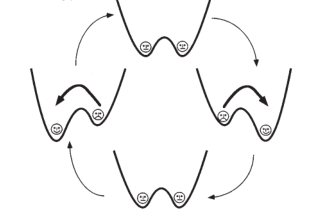
\includegraphics[width=20em]{000.png}
\caption{Transfer ratios on the Amazon benchmark. Both SDA-based systems outperforms the rest, and SDAsh (unsupervised training on all domains) is best.Reproduced from Glorot et al. (2011b).}
\label{fig:lable}
\end{figure}\\
\begin{equation}
\quad x'(t)=-V'(x)+A_0cos(wt+o)+u(t)
\end{equation}
\section{Related Work}
Until recently, most work on deep generative models focused on models that provided a parametric specification of a probability distribution function\cite{Eiber2013Attaining}. The model can then be trained by maximizing the log likelihood. In this family of model, perhaps the most succesful is the deep Boltzmann machine\cite{Pustejovsky1998The}.\\
\section{Adversarial nets}
The adversarial modeling framework is most straightforward to apply when the models are both multilayer perceptrons\cite{Wittrock1989Generative}. In the next section, we present a theoretical analysis of adversarial nets, essentially showing that the training criterion allows one to recover the data generating distribution as G and D are given enough capacity, i.e., in the non-parametric limit\cite{Yi2010Effective}.
.
{\small
\bibliographystyle{ieee}
\bibliography{1}
}
\end{document}
